\section{Results}

Some results I want to show.
\begin{itemize}
	\item Larger models tend to prefer parametric knowledge over contextual knowledge.
		\begin{itemize}
			\item This is the case in ``Characterizing Mechanisms for Factual Recall in Language Models'' \citep{factual_recall}, but I'm proving this on a larger set of question.
			\item This is using exact match. Maybe attempting Unigram F\textsubscript{1} would produce interesting results \citep{kilt}.
		\end{itemize}
	\item How this compares between Decoder-only models, Seq2Seq models, and Retrieval-Augmented Language Models.
	\item How does the perplexity between parametric answers and contextual answers compare within the same model.
		\begin{itemize}
			\item From the perplexity alone, can we predict whether an answer came from the model's memory or from the context?
			\item It might be worth experimenting this with factual answers in the context, to simulate a RAG-difference detector.
		\end{itemize}
	\item Is there any correlation between the perplexity of the parametric and contextual answer \textit{without any context} and which one will be chosen when adding context?
		\begin{itemize}
			\item This one is interesting, but I'm not sure we'll get significative results.
		\end{itemize}
	\item Interesting \textsl{``Other''} results.
	\item \textbf{Anything else}?
\end{itemize}

\subsection{Comparing the amounts of each type of answer}

\begin{figure}[h]
	\centering
	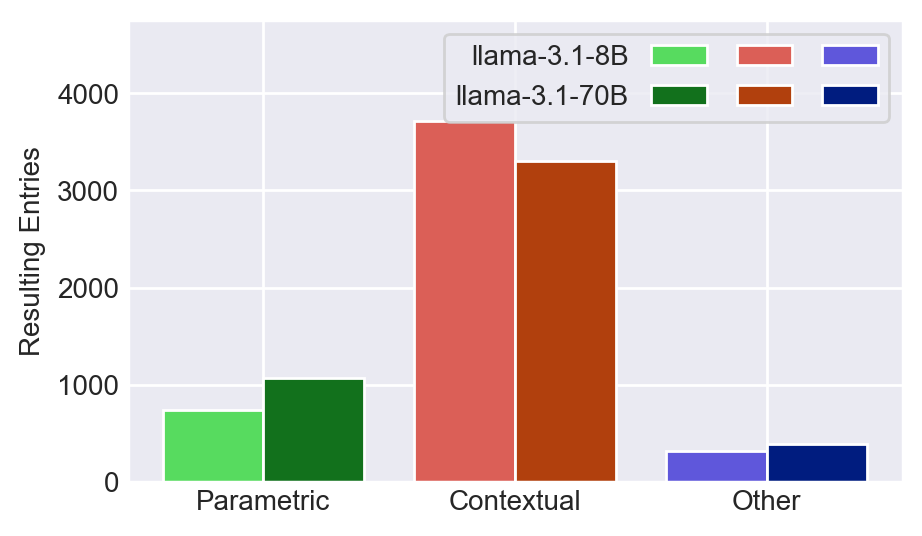
\includegraphics[width=.75\textwidth]{llama_amount.png}
	\caption{Amount of entries for each result after applying counterfactual context to Llama models. Generally, larger models tend to prefer parametric to contextual knowledge; this is further discussed in \cref{model_size_parametric}.}
\end{figure}

\begin{figure}[h]
	\centering
	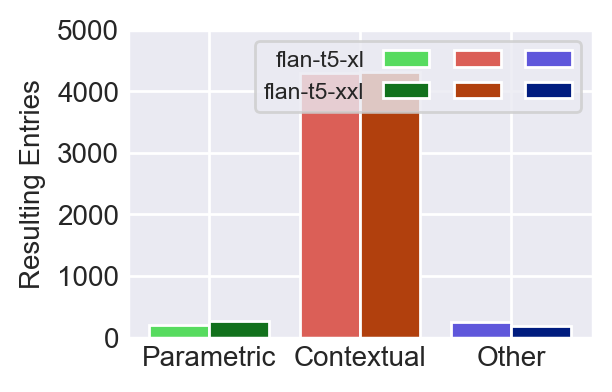
\includegraphics[width=.75\textwidth]{flan_amount.png}
	\caption{Same results for the Seq2Seq models \textsc{Flan-T5}. While these models tend to be more biased towards contextual knowledge, as discussed in \cref{model_type_parametric}, larger models still are biased towards parametric knowledge.}}
\end{figure}
